\documentclass[pdftex,12pt,a4paper]{article}

\usepackage{graphicx}  
\usepackage[margin=2.5cm]{geometry}
\usepackage{breakcites}
\usepackage{indentfirst}
\usepackage{pgfgantt}
\usepackage{pdflscape}
\usepackage{float}
\usepackage{epsfig}
\usepackage{epstopdf}
\usepackage[cmex10]{amsmath}
\usepackage{stfloats}
\usepackage{multirow}

\renewcommand{\refname}{REFERENCES}
\linespread{1.3}

\usepackage{mathtools}
%\newcommand{\HRule}{\rule{\linewidth}{0.5mm}}
\thispagestyle{empty}
\begin{document}
\begin{titlepage}
\begin{center}
\textbf{}\\
\textbf{\Large{ISTANBUL TECHNICAL UNIVERSITY}}\\
\vspace{0.5cm}
\textbf{\Large{COMPUTER ENGINEERING DEPARTMENT}}\\
\vspace{2cm}
\textbf{\Large{BLG 242E\\ DIGITAL CIRCUITS LABORATORY\\ EXPERIMENT REPORT}}\\
\vspace{2.8cm}
\begin{table}[ht]
\centering
\Large{
\begin{tabular}{lcl}
\textbf{EXPERIMENT NO}  & : & 2 \\
\textbf{EXPERIMENT DATE}  & : & 21.02.2020 \\
\textbf{LAB SESSION}  & : & FRIDAY - 15.30 \\
\textbf{GROUP NO}  & : & G4 \\
\end{tabular}}
\end{table}
\vspace{1cm}
\textbf{\Large{GROUP MEMBERS:}}\\
\begin{table}[ht]
\centering
\Large{
\begin{tabular}{rcl}
150170037  & : & SADIK MAHMUT \\
150180111  & : & MELİKE DOĞRAR   \\
150160117  & : & BUSE SİBEL KORKMAZ \\
\end{tabular}}
\end{table}
\vspace{2.8cm}
\textbf{\Large{SPRING 2020}}

\end{center}

\end{titlepage}

\thispagestyle{empty}
\addtocontents{toc}{\contentsline {section}{\numberline {}FRONT COVER}{}}
\addtocontents{toc}{\contentsline {section}{\numberline {}CONTENTS}{}}
\setcounter{tocdepth}{4}
\tableofcontents
\clearpage

\setcounter{page}{1}

\section{INTRODUCTION [10 points]}

In this experiment, we created the truth tables and made simplifications of the given expressions. Then we implemented this expressions on the CADET and compared the outputs to the results we expected.  

\section{MATERIALS AND METHODS [40 points]}
This experiment required usage of following equipments: CADET in order to implement the circuits of expressions, 74xx04 - Hex Inverter$^{1}$ to invert the inputs and sub-expressions. Also 74xx08 - Quadruple 2-input Positive AND Gates$^{1}$ and 74xx32 - Quadruple 2-input Positive OR Gates$^{1}$ are used to implement logic operations.

\subsection{PART 1}
In the first part of the experiment, logic circuits of the functions $F_1(a, b) = a + a \cdot b$ and $F_2(a, b) = (a + b) \cdot (a + b')$ examined and implemented on CADET. \\

The truth table and circuit of $F_1$ is below. 

\begin{table}[h]
    \centering
    \begin{tabular}{|c|c|c|c|}
    \hline
    a & b & $a \cdot b$ & a + $a \cdot b$ \\ \hline
    0 & 0 &       0     & 0         \\
    0 & 1 &       0     & 0         \\
    1 & 0 &       0     & 1         \\
    1 & 1 &       1     & 1         \\ \hline
    \end{tabular}
    \caption{Truth table of $F_1$}
    \label{fig1}
\end{table}

\begin{figure}[ht]
	\centering
	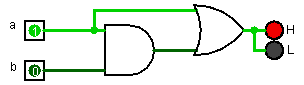
\includegraphics[width=0.5\textwidth]{2_1.png}	
	\caption{Circuit of $F_1$}
	\label{fig1}
\end{figure}

To implement the first expression, we used a 74xx08-AND Gate and a 74xx32-OR Gate. Firstly, we implemented $a \cdot b$ - which is a sub-expression of $F_1$ - by using an AND gate and for this, first we connected 0V to GND and +5V to GCC, then we connected $a$ to A1 and $b$ to B1 input pins and we took our output from Y1 pin. After that, by using an OR gate (we connected 0V to GND and +5V to GCC for that too), we brought $a$ and $a \cdot b$ (from Y1 output of AND gate) together. For that, we connected $a$ to A1 and $a \cot b$ to B1. Then we took $a + a \cdot b$ output from Y1. To check whether it's working or not, we connected the output to LED. What we expected was to see the changing of the LED's High and Low outcomes depending on input $a$ and we managed that. As a result of this experiment, as we can see in the truth table, we found that the whole function $F_1$ depends on input $a$.

The truth table and circuit of $F_2$ is below.

\begin{table}[h]
    \centering
    \begin{tabular}{|c|c|c|c|c|c|}
    \hline
    a & b & $b'$ & $a + b$ & $a + b'$ & $(a + b) \cdot (a + b')$ \\ \hline
    0 & 0 & 1    & 0       & 1        & 0                  \\
    0 & 1 & 0    & 1       & 0        & 0                  \\
    1 & 0 & 1    & 1       & 1        & 1                  \\
    1 & 1 & 0    & 1       & 1        & 1                  \\ \hline
    \end{tabular}
    \caption{Truth table of $F_2$}
    \label{fig2}
\end{table}

\begin{figure}[ht]
	\centering
	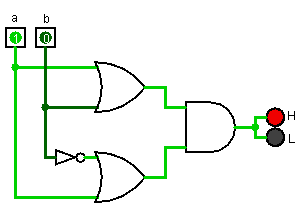
\includegraphics[width=0.5\textwidth]{2_1_2.png}	
	\caption{Circuit of $F_2$}
	\label{fig1}
\end{figure}
To implement the second expression, we used a 74xx04-Hex Inverter, a 74xx08-AND Gate and a 74xx32-OR Gate. Firstly, we implemented $a + b$ - which is a sub-expression of $F_2$ - by using an OR Gate and for this, first we connected 0V to GND and +5V to GCC, then we connected $a$ to A1 and $b$ to B1 input pins and we took our output from Y1 pin. After that, for the second part of the expression, we took the invert of $b$ first. To do that we used an inverter (to make the inverter work we connected 0V to GND and +5V to GCC). We connected $b$ to A1 as an input and we took $b'$ output from B1 pin. After that -by using the OR Gate again- we implemented $a + b'$ by connecting $a$ to A2 and $b'$ to B2 input pins and we took our output from Y2 output pin. At the end of all of this process, we got 2 outputs: $a + b$ and $a + b'$. Lastly, we brought these outputs together with AND Gate (to make the AND Gate work we connected 0V to GND and +5V to GCC) by connecting $a + b$ to A1 and $a + b'$ to B1 as inputs and we took our output from Y1. To check whether it's working or not, we connected the output to LED. What we expected was to see the changing of the LED's High and Low outcomes depending on input $a$ and we managed that. As a result of this experiment,as we can see in the truth table, we found that the whole function $F_2$ depends on input $a$.

\subsection{PART 2}
In this part of experiment, logic circuit is implemented for the dual of the given theorem ($a + a \cdot b = a$). To determine the dual of a boolean expression AND's replace with OR's and OR's replace with AND's. Thus, we found the dual of the given theorem $a \cdot (a + b)$. To implement this expression, we need an AND Gate and an OR Gate. First - to make them work - we connected 0V to  their GND and +5V to their GCC pins. After that, -by using an OR Gate- we implemented $a + b$. To do that we connected $a$ to A1 and $b$ to B1 pin of the OR Gate and we took our $a + b$ output from it's Y1 output pin. Then, we brought $a$ and $a + b$ together with AND Gate to implement $a \cdot (a + b)$. To do that we connected $a$ to A1 pin of the AND Gate and $a + b$ (from Y1 pin of the OR Gate) to B1 pin of the AND Gate. After that, we took our output from Y1 pin of the AND Gate and we connected it to two different LEDs. First one is to control the outcome of the expression and second one is to prove that the outcome depends on $a$ (and for that second LED is connect only to $a$). What we expected was to see the LEDs changing is parallel to each other and we managed to see that. So we validated the truth of the theorem. \\

The circuit of the dual of the theorem is below.
\begin{figure}[ht]
	\centering
	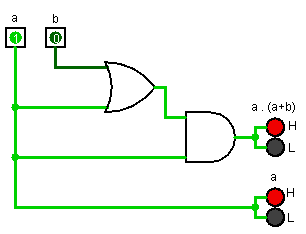
\includegraphics[width=0.5\textwidth]{2_2.png}	
	\caption{Circuit of $a \cdot (a + b)$}
	\label{fig1}
\end{figure}

\subsection{PART 3}
In the third part of the experiment, logic circuit is implemented for the complement of the given function ($F_3(a,b,c) = (a \cdot b) + (a' \cdot c)$ ). To determine the complement of a boolean expression AND's replace with OR's and OR's replace with AND's also variables replace with their inverses. When all these steps are done we found the complement of $F_3$ as $F_3'(a,b,c) = (a' + b') \cdot (a + c')$. To implement this expression, we need to use AND, OR Gates and and inverter. To make them work, we connected 0V to their GNDs and +5V to their GCCs. Firstly, we connected $a$ to A1 and $b$ to B1 input pins of the inverter. After that we took their outputs from Y1 and Y2. Then, we merged them with OR Gate. To do that, we connected the first output from the inverter to A1 and second output to B1. Thus, we implemented $(a' + b')$. Secondly, we connected $c$ to A3 input pin of the inverter to invert it. Then we took it's output from Y3 and merged it with $a$ by using OR Gate. To do that, we connected the output from Y3 pin of the inverter to A2 input pin of OR Gate and $a$ to B2 input pin of OR Gate. At the end of all this, we got two implemented expressions as $a'+b'$ and $a+c'$. What we need to do is bring them together with an AND Gate. To do that, we connected $a'+b'$ to A1 input pin of the AND Gate and $a+c'$ to B1 input pin. After that, we took the output from Y1 pin of the AND Gate and connected it to the LED. Then we tried all the combinations for inputs and we compared the outputs from our LED and truth table. In conclusion, we saw that our outputs and truth table matched without any failure. \\

The circuit and truth table of the complement of given function is below.

\begin{table}[h]
\centering
\begin{tabular}{|c|c|c|c|c|c|c|c|}
\hline
a & b & c & a' & $a \cdot b$ & $a' \cdot c$ & $F_{3}$ = $a \cdot b$ + $a' \cdot c$ & $F'_{3}$ \\ \hline
0 & 0 & 0 & 1  & 0     & 0      & 0                        & 1        \\ 
0 & 0 & 1 & 1  & 0     & 1      & 1                        & 0        \\ 
0 & 1 & 0 & 1  & 0     & 0      & 0                        & 1        \\ 
0 & 1 & 1 & 1  & 0     & 1      & 1                        & 0        \\ 
1 & 0 & 0 & 0  & 0     & 0      & 0                        & 1        \\ 
1 & 0 & 1 & 0  & 0     & 0      & 0                        & 1        \\
1 & 1 & 0 & 0  & 1     & 0      & 1                        & 0        \\ 
1 & 1 & 1 & 0  & 1     & 0      & 1                        & 0        \\ \hline
\end{tabular}
\caption{Truth table for $F_3$ and it's complement}
\label{fig3}
\end{table}

\begin{figure}[ht]
	\centering
	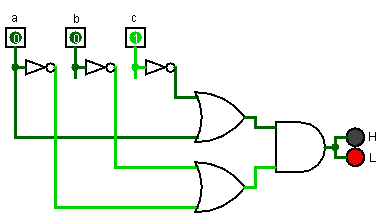
\includegraphics[width=0.5\textwidth]{2_3.png}	
	\caption{Circuit of $F_3'(a,b,c) = (a' + b') \cdot (a + c')$}
	\label{fig1}
\end{figure}

\subsection{PART 4}
In the last part of experiment, we simplified function $F_4(a,b,c,d) = U_1(1,2,5,6,9,10,13,14)$ and implemented it. We write the function in first canonical form to simplify :\\

$F_{4}(a,b,c,d) = (a'b'c'd) + (a'b'cd') + (a'bc'd) + (a'bcd') + (ab'c'd) + (ab'cd') + (abc'd) + (abc'd)$\\

To simplify the expression, we use axioms and theorems of boolean algebra :
\begin{align}
F_{4}(a,b,c,d) &= (a'b'c'd) + (a'b'cd') + (a'bc'd) + (a'bcd') + (ab'c'd) + (ab'cd') + (abc'd) + (abc'd) \notag\\ 
&= (a'b'c'd) + (a'bc'd) + (a'b'cd') + (a'bcd') + (ab'c'd) + (abc'd) + (ab'cd') + (abcd') \tag{Commutativity}\\
&= a'c'd(b' + b) + a'cd'(b'+b) + ac'd(b' + b) + acd'(b'+b) \tag{Distribution} \\
&= a'c'd(1) + a'cd'(1) + ac'd(1) + acd'(1) \tag{Inverse} \\
&= a'c'd + a'cd'+ ac'd+ acd' \tag{Identitiy} \\
&= a'c'd + ac'd + a'cd' + acd' \tag{Commutativity} \\
&= c'd(a' + a) + cd'(a' + a) \tag{Distribution} \\
&= c'd(1) + cd'(1) \tag{Inverse} \\
&= c'd + cd' \tag{Identity}
\end{align}

To implement this expression, we need to use 74xx04-Hex Inverter, a 74xx08-AND Gate and a 74xx32-OR Gate. To make them work, we connected 0V to their GNDs and +5V to their GCCs. First we did was inverting the $c$. To do that, we connected $c$ to the A1 input pin of the inverter and we took it's output from Y1 pin and merged this output with $d$ by using AND Gate. To do that, we connected the output from Y1 pin of inverter -which means $c'$ - to A1 input pin and $d$ to B1 input pin. Thus, we implemented $c' \cdot d$. The second thing we did was inverting the $d$. To do that, we connected $d$ to the A2 input pin of the inverter and we took it's output from Y2 pin and merged this output with $c$ by using AND Gate. To do that, we connected the output from Y2 pin of inverter -which means $d'$ - to A2 input pin and $c$ to B2 input pin. Thus, we implemented $c \cdot d'$. After this process, we got $c' \cdot d$ and $c \cdot d'$. What we did after that was getting them together with OR Gate. To do that, we connected $c' \cdot d$ to A1 input pin and $c \cdot d'$ to B1 input pin and we took the output from Y1 and connected it to the LED. We checked if the simplified expression matched the outcomes from LED or not and at the end of this, we saw that it was perfectly matched.

\begin{figure}[ht]
	\centering
	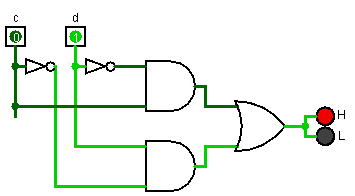
\includegraphics[width=0.5\textwidth]{2_4.png}	
	\caption{Circuit of simplified $F_4$}
	\label{fig1}
\end{figure}

\section{RESULTS}

As a result of this experiment, we learned this :
\begin{itemize}
    \item When you get the dual of both sides of an equivalence, the equivalence does not break.
    \begin{itemize}
        \item $a + a \cdot b = a$
        \item $a \cdot (a + b) = a$
    \end{itemize}
    \item How to implement XOR Gate using 74xx04-Hex Inverter, 74xx32-OR Gate and 74xx08-AND Gate
    \item How to take a complement of an expression
    \item What is the absorption rule and how to use it
\end{itemize}



\section{DISCUSSION}
In order to prepare to the lecture, first we did was, we revised the axioms and theorems of Boolean algebra$^{2}$. After that, we made sure that our 74xx04-Hex Inverter, 74xx32-OR Gate, 74xx08-AND Gate, cables and C.A.D.E.T was ready to work.\\

Then we started to Part 1 of the experiment. We did all the steps we mentioned above for Part 1.
The aim of Part 1 was to prove the Absorption rule we learnt in Digital Circuits lectures by making a physical experiment with real Gates and C.A.D.E.T.\\

After that we started to Part 2 of the experiment. We also did all the steps we mentioned above for Part 2. The aim of Part 2 was to learn how to determine the dual of an expression. Therefore we learnt it and implemented the expression by using C.A.D.E.T. and Gates.\\

After that we started to Part 3 of the experiment. We also did all the steps we mentioned above for Part 3. The aim of Part 3 was to learn how to take the complement of an expression. Therefore, we learnt it and implemented the expression by using C.A.D.E.T. and Gates. Finally, we design truth table of expression and compared it outcomes of expression we implemented on C.A.D.E.T.\\

Lastly, we started to Part 4 of the experiment. We also did all the steps we mentioned above for Part 4. The aim of Part 4 was to learn how to simplify expressions. To do that, we revised the axioms and theorems of Boolean algebra. After that, we implemented the expression on C.A.D.E.T. that we simplified with using Boolean algebra

\section{CONCLUSION}
Since we worked a little messy at the beginning of the experiment, we did not notice a cable that we plugged in incorrectly. That's why we learned to work more carefully during the experiment. Other than that, we did not encounter any difficulties.


\newpage
\addcontentsline{toc}{section}{\numberline {}REFERENCES}

\bibliographystyle{unsrt}
\bibliography{reference}\\

[1]Istanbul Technical University Department of Computer Engineering. BLG 242E Logic Circuits Laboratory Experiments Booklet, version 1.9.1, Spring 2020.\\

[2]Istanbul Technical University Department of Computer Engineering. BLG 231E Digital Circuits Lecture Slides. https://ninova.itu.edu.tr/en/courses/faculty-of-computer-and-informatics/1591/blg-231e/ekkaynaklar/.\\

[3] Overleaf documentation https://tr.overleaf.com/learn.
\end{document}

